\documentclass[11pt,twoside]{report}
\usepackage{geometry}
\usepackage{enumerate}
\usepackage{latexsym,booktabs}
\usepackage{amsmath,amssymb}
\usepackage{graphicx}
\usepackage[singlespacing]{setspace}
% ===== Defaults^
\usepackage{amsthm}
\usepackage{hyperref}           % hyperlinks
\usepackage{array}              % for \newcolumntype macro
\usepackage[ruled,vlined,linesnumbered]{algorithm2e}
\usepackage{mathtools}
\usepackage{tikz}
\usepackage{mathrsfs} %% mathscr for powerset

%TC:ignore
\newcolumntype{C}{>{$}c<{$}}    % math-mode version of "l" column type
\newcolumntype{L}{>{$}l<{$}} 
%TC:endignore

\newcommand{\A}{\mathcal{A}} %% I am lazy
\newcommand{\K}{\mathcal{K}}
\newcommand{\norm}[1]{\left\lVert#1\right\rVert} % norm
\newcommand{\binary}{\left\{0,1\right\}} % lazy

\DeclareMathOperator{\MEB}{MEB}
\DeclareMathOperator{\MEBwO}{MEBwO}

\DeclarePairedDelimiter\ceil{\lceil}{\rceil}
\DeclarePairedDelimiter\floor{\lfloor}{\rfloor}

\theoremstyle{definition}

\usetikzlibrary{shapes.misc} % crosses
\tikzset{cross/.style={cross out, draw=black, minimum size=2*(#1-\pgflinewidth), inner sep=0pt, outer sep=0pt},
%default radius will be 1pt. 
cross/.default={2pt}}
% ==== Mine^

\geometry{a4paper,left=2cm,right=2.0cm, top=2cm, bottom=2.0cm}

\newtheorem{definition}{Definition}
\newtheorem{theorem}{Theorem}
\newtheorem{lemma}{Lemma}
\newtheorem{corollary}{Corollary}
\newtheorem{proposition}{Proposition}
\newtheorem*{remark}{Remark}
\numberwithin{theorem}{section}
\numberwithin{definition}{section}
\numberwithin{lemma}{section}
\numberwithin{proposition}{section}
\numberwithin{equation}{section}
\numberwithin{figure}{section}


\begin{document}
\pagestyle{empty}

% =============================================================================
% Title page
% =============================================================================
\begin{titlepage}
\vspace*{.5em}
\center
\textbf{\large{The School of Mathematics}} \\
\vspace*{1em}
\begin{figure}[!h]
\centering

\includegraphics[width=180pt]{CentredLogoCMYK.jpg}
\end{figure}
\vspace{2em}
\textbf{\Huge{Minimum Enclosing Balls with Outliers}}\\[2em]
\textbf{\LARGE{by}}\\
\vspace{2em}
\textbf{\LARGE{Thomas Holmes}}\\
\vspace{6.5em}
\Large{Dissertation Presented for the Degree of\\
MSc in Operational Research with Computational Optimization}\\
\vspace{6.5em}
\Large{August 2021}\\
\vspace{3em}
\Large{Supervised by\\Dr E. Alper Yıldırım}
\vfill
\end{titlepage}

\cleardoublepage

% =============================================================================
% Abstract, acknowledgments, and own work declaration
% =============================================================================
\vspace*{10mm}
\begin{center}
\textbf{\huge{Abstract}}
\end{center}

Here comes your abstract ...

\clearpage
\vspace*{10mm}
\begin{center}
\textbf{\huge{Acknowledgments}}
\end{center}

Here come your acknowledgments ...

\clearpage

\vspace*{10mm}
\begin{center}
\textbf{\huge{Own Work Declaration}}
\end{center}
\vspace*{20mm}

\noindent I declare that this thesis was composed by myself and that the work contained therein is my own, except where explicitly stated otherwise in the text.

\vspace*{10mm}

\begin{flushright}
\textit{(Thomas Holmes)}
\end{flushright}

\cleardoublepage



% =============================================================================
% Table of contents, tables, and pictures (if applicable)
% =============================================================================
\pagestyle{plain}
\setcounter{page}{1}
\pagenumbering{Roman}

\tableofcontents
\clearpage
\listoftables
\listoffigures
\cleardoublepage

\pagenumbering{arabic}
\setcounter{page}{1}

\nocite{*}
\bibliographystyle{abbrv}
\clearpage
% =============================================================================
% Main body
% =============================================================================

% =============================================================================
% Chapter 1
% =============================================================================
\chapter{Introduction}
\section{Motivation}
\section{Outline}

% =============================================================================
% Chapter 2
% =============================================================================
\chapter{Problem Definition and Literature Review}\label{exact}
\section{Preliminaries}
In this paper we shall denote our data set of finite vectors as $\mathcal{A} = \left\{a^1,\ldots,a^n\right\}\subseteq\mathbb{R}^d$ for $n,d\in\mathbb{N}$. The center of a ball is represented by a vector $c\in\mathbb{R}^d$, the radius a scalar $r\in\mathbb{R}$, and the squared radius $\gamma=r^2$. We denote the percentage of inliers for a minimum enclosing ball with outliers (MEBwO) by $\eta\in(0,1]$, i.e. if $\eta=0.9$ then we seek a ball which covers $90\%$ of our data. While it may be easier for us to think practically of the MEBwO as covering $\eta\%$ of our data, it is easier mathematically to consider a MEBwO which covers $n-k$ out of $n$ data points, where $k=\floor{n(1-\eta)}$ is the number of outliers.

We would now like to make some formal definitions.

\begin{definition}
    Let $c\in\mathbb{R}^n$ and $r\in\mathbb{R}$. Then the \textit{ball} with center $c$ and radius $r$ is the set
    \begin{equation*}
        B(c;r) = \left\{x\in\mathbb{R}^n : \norm{x-c} \leq r\right\}
    \end{equation*}
    where $\norm{\cdot}:L\to\mathbb{R}$ denotes the standard Euclidean norm on a vector space $L$ (in this paper, $L=\mathbb{R}^n$).
\end{definition}

\begin{definition}
    The \textit{minimum enclosing ball} of $\A$, denoted by $\MEB(\A)$, is the ball $B(c^*,r^*)$ where $\A\subseteq B(c^*,r^*)$ and if any $B(c,r)$ exists such that $\mathcal{A}\subseteq B(c,r)$ then $r^*\leq r$.
\end{definition}

\begin{theorem}\label{thm:unique}
    For a given set $\A$, $\MEB(\A)$ exists and is unique.
\end{theorem}
\begin{proof}
    See \cite[page 5]{two-algorithms}.
\end{proof}

Now, we are interested in the idea that adding or removing data from a data set may have an effect on the radius of the MEB of that data set.
\begin{proposition}\label{adding data}
    Let $a'\in\mathbb{R}^n$ where $a'\notin\A$. Suppose $B(c,r)=\MEB(\A)$ and $B(c',r')=\MEB(\A\cap\left\{a'\right\})$. Then $r\leq r'$.
\end{proposition}
\begin{proof}
    Clearly we have $\A\subseteq\A\cap\left\{a'\right\}$, then since $\A\cap\left\{a'\right\}\subseteq B(c',r')$ we have $\mathcal{A}\subseteq B(c',r')$ by transitivity. Thus $r\leq r'$ with equality only if $a'\in B(c,r)$ by uniqueness.
\end{proof}

\begin{proposition}\label{removing data}
    Suppose $a'\in\A$. Let $B(c,r)=\MEB(\A)$, $B(c',r')=\MEB(\A\setminus\left\{a'\right\})$. Then $r'\leq r$.
\end{proposition}
\begin{proof}
    Clearly we have $\A\setminus\left\{a'\right\}\subseteq\A$ then since $\A\setminus\left\{a'\right\}\subseteq B(c',r')$ and $\A\setminus\left\{a'\right\}\subseteq B(c,r)$ we have $r'\leq r$ since $B(c',r')$ is the MEB for $\A\setminus\left\{a'\right\}$, with equality only if $\MEB(\A\setminus\left\{a'\right\} = \MEB(\A)$ by uniqueness.
\end{proof}
These two propositions tell us that when we add data to a set, the resulting MEB is either unchanged or bigger. Conversely, when we remove data from a set, the resulting MEB is either unchanged or smaller.

In the interest of contextualizing Algorithm \ref{core-set algorithm}, we define the $(1+\epsilon)$-approximation to an MEB and core-sets.
\begin{definition}[{{\cite[page 2]{core-sets}}}]
    Let $\epsilon>0$. Let $r^*$ be the radius of $\MEB(\A)$. A ball $B(c;(1+\epsilon)r)$ is a \textit{$(1+\epsilon)$-approximation} of $\MEB(\A)$ if $r\leq r^*$ and $\mathcal{A}\subseteq B(c,(1+\epsilon)r)$.
\end{definition}

\begin{definition}[{{\cite[page 2]{core-sets}}}]
    Let $\epsilon>0$. A subset $X\subseteq\A$ is a \textit{$\epsilon$-core-set} (typically just referred to as a \textit{core-set}) of $\A$ if $\A\subset B(c,(1+\epsilon)r)$.
\end{definition}
Finally, the following two definitions allow us to formally define the MEBwO.
\begin{definition}
    For a set $\A$, the set of $k$-subsets of $\A$ is the set $\mathfrak{K}=\left\{\K\in\mathscr{P}(\A): |\K|=k\right\}$ where $\mathcal{P}:\textbf{Set}\to\textbf{Set}$ is the usual power set functor.
\end{definition}

\begin{definition}
    For some $\eta\in[0,1]$, let $k=\floor{n(1-\eta)}$ be the number of outliers in $\A$. Then the \textit{minimum enclosing ball with outliers} of $\A$, denoted by $\MEBwO(\A,\eta)$, which covers $\eta\%$ of $\A$, is the ball $B(c^*,r^*)=\MEB(\K^*)$ for $\K^*\in\mathfrak{K}$ a $k$-subset of $\A$ where for all other $k$-subsets $\K\in\mathfrak{K}$, $\K\neq\K^*$, if $B(c,r)=\MEB(\K)$ then $r^*\leq r$.
\end{definition}

We may deduce that for a given data set $\A$, an MEBwO exists since an MEBwO is simply the MEB of some $k$-subset of $\A$, which by Theorem \ref{thm:unique} exists and is unique for that $k$-subset. However, MEBwO's are not unique. 

For a simple example, consider the data set $\A=\left\{(-2,-1),(2,-1),(2,1),(-2,1)\right\}$ with $\eta=\frac{1}{2}$. Then $B((-2,0),1)$ and $B((2,0),1)$ are both MEBwO's for $\A$, and MEB's for the $2$-subsets $\left\{(-2,-1), (-2,1)\right\}$, $\left\{(2,-1), (2,1)\right\}$ of $\A$ respectively. See Figure \ref{fig:mebwo non-unique} for a visualisation of this example.

\begin{figure}
    \centering
    \begin{tikzpicture}
        % axes
        \draw[<->] (0, -2.5) -- (0,2.5);
        \draw[<->] (-3.5, 0) -- (3.5, 0);
        
        % points
        \foreach \coord in {(-2,-1), (2,-1)}{
            \draw[fill] \coord circle (1.5pt) node[below]{\coord};
        }
        \foreach \coord in {(2,1), (-2,1)}{
            \draw[fill] \coord circle (1.5pt) node[above]{\coord};
        }
        
        % balls
        \foreach \coord in {(-2,0), (2,0)}{
            \draw \coord circle (1);
            \draw \coord node[cross, red]{};
        }
        
    \end{tikzpicture}
    \caption{Example of MEBwO non-uniqueness}
    \label{fig:mebwo non-unique}
\end{figure}

\section{Minimum Enclosing Ball}
\begin{definition}\label{meb}
    The optimization model formulation of the Minimum Enclosing Ball (MEB) problem is as follows:
    \begin{center}
        \begin{tabular}{CCC}
            \displaystyle\min_{c,r} & r \\
            \text{s.t.} & \norm{c-a^i} \leq r & i=1,\ldots,n
        \end{tabular}
    \end{center}
    where $c\in\mathbb{R}^d$ and $r\in\mathbb{R}$ are the decision variables corresponding to the center and radius of the ball respectively.
    
    As detailed in \cite{two-algorithms}, the MEB problem can be transformed to a convex quadratic problem (QP) by squaring the constraints and defining a new decision variable $\gamma=r^2$:
    
    \begin{center}
        \begin{tabular}{CLC}
            \displaystyle\min_{c,\gamma} & \gamma \\
            \text{s.t.} & \left(a^i\right)^Ta^i - 2\left(a^i\right)^Tc + c^Tc \leq \gamma & i=1,\ldots,n
        \end{tabular}
    \end{center}
\end{definition}
This problem has $d+1$ variables and $n$ constraints, which can make it slow to find an optimal solution by using a solver such as Xpress or Gurobi, but many alternative approaches are present in the literature which offer very fast solutions within a guaranteed accuracy (\cite{core-sets}, \cite{two-algorithms}).

We will discuss here one such algorithm to solve the MEB problem from \cite{core-sets} that will be used in algorithms in Chapter \ref{algorithms}. The central idea is that of the \textit{core-set} \cite{agarwal2005geometric}, which is a small set of points that approximate the shape of a larger set of points. For example, a circle can be represented by a core-set of three points which lie on the boundary of the circle.

%TODO: image of 2d circle with core-set here

The idea of the algorithm is to create a candidate core-set, check if the MEB of this core-set contains all of the input data, and if so return the MEB, if not grow the core-set by adding the furthest point from the center of the candidate MEB. For further details please see \cite{core-sets}.

\begin{algorithm}[H]\label{core-set algorithm}
    \SetAlgoLined
    \KwIn{Data set $\A=\left\{a^1,\ldots,a^n\right\}$, error tolerance $\epsilon>0$}
    \KwOut{$(1+\epsilon)$-approximation to $\MEB(\A)$ and an $O(1/\epsilon)$-size core-set}
    
    Let $p$ be any point in $\A$ (can be chosen randomly)\;
    $q=\arg\max_{a\in\A}\norm{p-a}$\;
    $q'=\arg\max_{a\in\A}\norm{q-a}$\;
    $X := \left\{q,q'\right\}$\;
    $\delta := \epsilon^2/163$\;
    \While{True}{
        Let $B(c',r')$ denote the $(1+\delta)$-approximation to $\MEB(X)$ returned by solver\;
        \eIf{$\A\subseteq B(c',(1+\epsilon/2)r'$}{
            break\;
        }{
            $p:=\arg\max_{a\in\A}\norm{a-X}$
        }
        $X := X\cup\left\{a\right\}$
    }
    \KwRet $B(c',(1+\epsilon/2))$, $X$
    \caption{Core-Set Algorithm for the MEB Problem \cite{core-sets}}
\end{algorithm}

Algorithm \ref{core-set algorithm} runs in $O\left(\frac{nd}{\epsilon}+\frac{d^2}{\epsilon^{3/2}}\left(\frac{1}{\epsilon}+d\right)\log\frac{1}{\epsilon}\right)$ time \cite[Page 6]{core-sets}.

\section{Minimum Enclosing Ball with Outliers}
\subsection{Formulation}
\begin{definition}\label{mebwo}
    We may extend Definition \ref{meb} to the Minimum Enclosing Ball with Outliers (MEBwO) problem as follows:
    \begin{center}
        \begin{tabular}{CCC}
             \displaystyle\min_{c,r,\xi} & r \\
             \text{s.t.} & \norm{c-a^i} \leq r + M\xi_i & i=1,\ldots,n \\
             & \displaystyle\sum_{i=1}^n\xi_i \leq k \\
             & \xi_i \in \binary & i=1,\ldots,n
        \end{tabular}
    \end{center}
    
    where $\xi_i$ are binary variables corresponding to the distance constraint on each variable, with $M\in\mathbb{R}$ a sufficiently large scalar. One can interpret this as, if $\xi_i=1$ for some $i\in\left\{1,\ldots,n\right\}$, then $a_i$ does not need to be inside the ball. The constraint $\sum_{i=1}^n\xi_i\leq k$ where $k=\floor{n(1-\eta)}$ ensures that $\eta\%$ of the data is covered.
    
    We can instead extend the quadratic program in Definition \ref{meb} to get the following mixed integer quadratic program formulation:
    \begin{center}
        \begin{tabular}{CLC}
            \displaystyle\min_{c,\gamma, \xi} & \gamma \\
            \text{s.t.} & \left(a^i\right)^Ta^i - 2\left(a^i\right)^Tc + c^Tc \leq \gamma + M\xi_i & i=1,\ldots,n \\
            & \displaystyle\sum_{i=1}^n\xi_i \leq k \\
            & \xi_i \in \binary & i=1,\ldots,n
        \end{tabular}
    \end{center}
\end{definition}
\begin{remark}
    One may note that when we relax $\xi_i$ to be continuous variables, i.e. $0\leq\xi_i\leq1$ for $i=1,\ldots,n$, we have again a convex quadratic program since we have then added only continuous variables and linear constraints to the base quadratic program.
\end{remark}

This model gives us a way to solve the MEBwO problem optimally for a given data set. However, by examining the structure of this model we can expect the solution times to be unreasonable for any meaningfully large instance. Note that, of $n$ many binary variables $\xi_i$, we can choose up to $k\leq n$ many of them to have a value of 1, though by Proposition \ref{removing data} we know that removing data gives us an MEB with potentially lower radius, meaning we will always pick the highest possible number of points ($k$ many) to be excluded. Thus, by a total brute force search we may expect to explore $\binom{n}{k}$ many individual MEB problems. Modern optimization solvers will work more efficiently than this, utilizing techniques such as branch-and-bound (first proposed by \cite{bnb}). Regardless, we expect a very large solution space which leads to exponentially larger solution times as we will see in Section \ref{exact benchmarks}.


\subsection{On the Big M Parameter}
The ``big $M$ constraint" in Definition \ref{mebwo} is a commonly known technique within Operational Research and an important question is that of what $M$ do we choose? A sufficiently large $M$ is required such that when the corresponding binary variable is equal to $1$, the constraint is effectively nullified. But, as we will see within this section, a value of $M$ which is too large will lead to a less effective model.
\subsubsection{Solution Times}
One concern with our choice of $M$ is the effect on the solution time of the solver.

\subsubsection{An Upper Bound on $M$}
Finding a suitable value of $M$ depends heavily on the nature of the problem the constraint is being applied to. For the minimum enclosing ball with outliers problem, where we are concerned with the distances $\norm{c-a^i}$ being less than the radius $r$, we look to add a value to $r$ such that for any reasonable $c$, this constraint is always satisfied. Thus, a candidate upper bound for $M$ may be found by calculating each pairwise distance within the data and recording the largest distance. Formally, this may be written as $M:= \max\left\{\norm{a^i-a^j}: i,j = 1,\ldots,n, i\neq j\right\}$.

An immediately apparent issue with this approach is that computing $M$ in this way will run in $O(n^2d)$ time. For smaller data sets this is manageable, but for any significantly sized data sets the time taken to compute $M$ is often longer than the time taken to solve the MEBwO problem on the same data. 

We can look to \cite[Page 4]{core-sets} for a $1/\sqrt{3}$-approximation to the diameter of $\A$ which runs in $O(nd)$ time, by picking a random point $p\in\A$, then computing $q=\arg\max_{a\in\A}\norm{p-a}$ and $q'=\arg\max_{a\in\A}\norm{q-a}$, i.e. $q$ the furthest point from $p$ and then $q'$ the furthest point from $q$. Then we set $D:=\norm{q-q'}$ which is our $1/\sqrt{3}$-approximation to the diameter of $\A$. 
\subsubsection{Quality of $\xi_i$ Solutions in the QP Relaxation}
Another concern regarding the value of $M$ is the effect on the optimal solutions for the relaxed $\xi_i$ variables in the QP relaxation. This is important as good quality relaxed solutions are essential to Algorithm \ref{relaxation heuristic}.

\section{Literature Review}\label{lit review}

% =============================================================================
% Chapter 3
% =============================================================================

\chapter{Heuristic and Approximation Algorithms}\label{algorithms}

In this chapter we propose some non-exact construction methods to solving the MEBwO problem which return a feasible solution. We also investigate some improvement heuristics which, given a feasible MEB or MEBwO, seek to locally find a new center such that a smaller radius can be found.

\section{Construction Methods}
\subsection{Relaxation-Based Heuristic}
This heuristic works by first solving the relaxed QP formulation for the MEBwO problem in Definition \ref{mebwo}, and then making the assumption that a higher value of $\xi_i$ (i.e. closer to 1) means that the model treats the data point $a^i$ as ``more" of an outlier. From this assumption, we pick the largest $k$ values of $xi_i$ and treat each corresponding $a^i$ as an outlier, therefore treating the remaining data as inliers. We then solve the MEB problem for this remaining data. A more formal outline of this algorithm is detailed in Algorithm \ref{relaxation heuristic}.

This method will always return a feasible solution that covers $\eta\%$ of the data as we will always remove $k=\floor{n(1-\eta)}$ many points. As discussed in the previous chapter, solving the final MEB problem is relatively easy and selecting outliers using the MEBwO QP relaxation is trivial, but the difficulty lays in solving the initial QP relaxation, and as such a heuristic method which can solve this model quickly and return approximate solutions to each $xi_i$ is a valuable direction for further research in order to speed up this method.

\begin{algorithm}[H]\label{relaxation heuristic}
    \SetAlgoLined
    \KwIn{Data set $\A=\left\{a^1,\ldots,a^n\right\}$, percentage of data to be covered $\eta\in[0,1]$, error tolerance for MEB heuristic $\epsilon>0$, big $M$ parameter $M>0$}
    \KwOut{Ball $B(c,r)$}
     $\xi=\left[\xi_1,\ldots,\xi_n\right]$ relaxed binary variables returned by relaxed MEBwO solver for $\A$, $\eta$, and $M$\;
     Let $\xi'$ be the smallest $k=\floor{\eta\cdot n}$ elements of $\xi$\;
     Let $\A':=\left\{a^i\in\A: \xi_i\in\xi',\ i=1,\ldots,n\right\}$\;
     Let $c,r$ be the center and radius of $\MEB(\A')$ returned by heuristic\;
     \KwRet $B(c, r)$\;
     
    \caption{Relaxation-Based Heuristic}
\end{algorithm}
\subsection{Shrinking Heuristics}
These heuristics work by computing a candidate centre for the ball, then computing the $k$ closest points and returning the ball $B(c,r)$ where $r$ is the maximum distance from $c$ to each of the $k$ closest points.

\subsubsection{MEB Shrinking Heuristic}
Our first shrinking heuristic finds a candidate centre by first computing $\MEB(\A)=B(c,r')$, then finding the $k$ closest points and returning the ball $B(c,r)$ as described above.

\begin{algorithm}[H]\label{meb shrink}
    \SetAlgoLined
    \KwIn{Data set $\A$, $\eta\in[0,1]$, $\epsilon>0$}
    \KwOut{Ball $B(c,r)$}
    $k:=\floor{n(1-\eta)}$\;
    Let $c$ be the center of the MEB returned by a heuristic for $\MEB(\A)$\;
    $D:=\left\{\norm{c-x}: x\in\A\right\}$\;
    Let $D'$ be $D$ sorted in ascending order\;
    Let $\delta$ be the $(k-1)$th element of $D'$ (indexing from 0)\;
    $\A' = \left\{a^i\in\A: D[i] \leq \delta, i=1,\ldots,n\right\}$\;
    $r = \max_{a\in\A'}\norm{c-a}$\;
    \KwRet $B(c,r)$\;
    
    \caption{MEB Shrinking Heuristic}
\end{algorithm}

\subsubsection{Average Point Shrinking Heuristic}
Our second heuristic finds a candidate centre by simply finding the average point, i.e. $c=\frac{1}{n}\sum_{i=1}^n a^i$, then finding the $k$ closest points and returning the ball $B(c,r)$ as described above.

\begin{algorithm}[H]\label{avg point shrink}
    \SetAlgoLined
    \KwIn{Data set $\A$, $\eta\in[0,1]$}
    \KwOut{Ball $B(c,r)$}
    $k:=\floor{n(1-\eta)}$
    $c:=\frac{1}{n}\sum_{i=1}^na^i$\;
    $D:=\left\{\norm{c-x}: x\in\A\right\}$\;
    Let $D'$ be $D$ sorted in ascending order\;
    Let $\delta$ be the $(k-1)$th element of $D'$ (indexing from 0)\;
    $r = \max_{a\in\A'}\norm{c-a}$\;
    \KwRet{$B(c,r)$}
    
    \caption{Average Point Shrinking Heuristic}
\end{algorithm}
\subsection{Shenmaier's Approximation}
\subsubsection{Statement}
This approximation scheme developed by Vladimir Shenmaier in \cite[Algorithm 1]{SHENMAIER201581} is a brute-force algorithm to solving the MEBwO problem with $O(n^2d)$ time complexity. It works by considering each point in the input set, finding the $k$-closest points to that point, then returning the point-distance pair such that the maximum distance from each point to each other point in its $k$-closest points is minimised. See Algorithm \ref{shenmaier} for a detailed outline of this algorithm.
\begin{algorithm}\label{shenmaier}
    \KwIn{Data set $\A$, $\eta\in[0,1]$}
    \KwOut{Ball $B(c,r)$}
    $k=\floor{n(1-\eta)}$\;
    \For{$i=1,\ldots,n$}{
        $D:=\left\{\norm{c-a}: a\in\A\right\}$\;
        Let $D'$ be $D$ sorted in ascending order\;
        Let $\delta_i$ be the $(k-1)$th element of $D'$ (indexing from 0)\;
    }
    $i^* := \arg\min_{i=1,\ldots,n}\delta_i$\;
    $c := a^{i^*}$\;
    $r := \delta_{i^*}$\;
    \KwRet{$B(c,r)$}\;
    
    \caption{Shenmaier's Approximation \cite[Algorithm 1]{SHENMAIER201581}}
\end{algorithm}
\subsubsection{Approximation Guarantee}
 From \cite[Theorem 4]{SHENMAIER201581} we know that Algorithm \ref{shenmaier} returns a 2-approximation solution to the MEBwO problem. What this means is that if we have a minimum radius of $r$ returned by Algorithm \ref{shenmaier} for a data set $\A$, then the true optimal value to the MEBwO problem on that data is no less than $r/2$. This is useful for assessing how close a heuristic is to an optimal solution in the worst case when we have a solution via Algorithm \ref{shenmaier}, but not an optimal solution via solving the exact model.

\subsubsection{Complexity}
Referring to Algorithm \ref{shenmaier}, on line 1 we have an assignment which runs in $O(1)$ time. On lines 2 through 5 we have a \texttt{for} loop which runs $n$ many times, and on line 3 we compute a list of $n$ many distances, which for $d$-dimensional vectors runs in $O(nd)$ time. Line 4 involves sorting the aforementioned list, so the time complexity depends on the sorting algorithm used. It is well known within computer science that algorithms are often subject to a time-memory trade off, meaning that it is possible to design algorithms that run faster as a result of using less memory, and vice-versa. We can then assume that a sensible implementation of Algorithm \ref{shenmaier} would use the fastest available sorting algorithm given that the size of our data sets are small enough that we do not run into memory constraints, so the recommended sorting algorithm is Quicksort \cite{hoare1962quicksort} which runs on average in $O(n\log n)$ time. Line 5 simply accesses the $(k-1)$th element of the sorted list and so runs in $O(1)$ time.

Line 6 finds the minimum element from a set of values and runs in $O(n)$ time. Lines 7 and 8 are simple assignments and run in $O(1)$ time. Finally, our overall time complexity is then $O(n^2(d+\log n))$. This will usually reduce to $O(n^2d)$ as typically $d>\log n$, though for particularly large $n$ and very small $d$ the alternative reduction of $O(n^2\log n)$ is of course possible.
\section{Improvement Heuristics}
We now consider some improvement heuristics. The two heuristics described here are, strictly speaking, designed to improve an existing MEB rather than an MEBwO. However, quick and effective methods exist for solving the MEB problem and so improvement heuristics have not been needed, while heuristics which solve the MEBwO problem may return a solution which has considerable space for improvement.

The two improvement heuristics work in a similar way, by considering an improving direction in which moving the centre of the MEB in that direction while keeping the same radius retains a feasible solution, then shrinking the radius to the furthest point from the new centre. The Direction-Constrained Single Step Heuristic (DCSSH) works by pure geometric reasoning to find a new centre, while the Direction-Constrained MEB (DCMEB) uses an optimization solver such as Gurobi to find an optimal step in the improving direction to minimize the radius of the new ball.

The inspiration for these heuristics comes from Shenmaier's Approximation, which returns a ball with some centre $c\in\A$. Our assumption is that a better solution exists in a local neighbourhood around $c$, i.e. we find a new centre that does not have to lie on a point in $\A$.

\subsection{Direction-Constrained Single Step Heuristic}
\subsubsection{Derivation}
For a visual aid to this derivation please refer to Figure \ref{vis aid derivation}. Consider $B(\hat{c}, r) = \MEB(\A)$. To find an improving direction we choose the furthest point from $c$, $\hat{a}=\arg\max_{a\in\A}\norm{c-a}$, then the (negative) improving direction is defined to be $\beta=\hat{c}-\hat{a}$. We choose the direction $\hat{a}\to\hat{c}$ as opposed to $\hat{c}\to\hat{a}$ in order to simplify later derivations.

Now that we have a direction $\beta$, we can move the initial ball in this direction by simply subtracting $\beta x$ from $\hat{c}$ where $x\in\mathbb{R}^{\geq0}$ is some scalar, i.e. our new centre is $c=\hat{c}-\beta x$. We would like to choose $x$ such that the new ball remains feasible by ensuring that $\norm{c-a^i}\leq r$ for $i=1,\ldots,n$, and we can do this by considering the distance from each $a^i$ in the direction of $\beta$ to the surface of the initial ball and choose $x$ such that each of these distances is greater than $\norm{\beta x}$.

More formally, for each $a^i\in\A$ let $x_i$ be the scalar such that $a^i+\beta x_i$ lies on the surface of the initial ball, i.e. $\norm{(a^i+\beta x^i)-\hat{c}}=r$. Again, to simplify derivations, denote the direction $\hat{c}\to a^i$ by $\alpha_i=a^i-\hat{c}$. To calculate each $x_i$, we square this equation and set $\gamma=r^2$ to get
\begin{align*}
    \alpha_i^T\alpha_i + 2x\alpha_i^T\beta + x^2\beta^T\beta &= \gamma \\
    \implies \beta^T\beta x^2 + 2\alpha_i^T\beta x + \alpha_i^T\alpha_i - \gamma &= 0.
\end{align*}
Using the quadratic formula we then have
\begin{align*}
    x &= \frac{-2\alpha_i^T\beta \pm \sqrt{4\left(\alpha_i^T\beta\right)^2 - 4\beta^T \beta\left(\alpha_i^T\alpha_i-\gamma\right)}}{2\beta^T\beta} \\[4pt]
    &= \frac{-\alpha_i^T\beta \pm \sqrt{\left(\alpha_i^T\beta\right)^2 - \beta^T \beta\left(\alpha_i^T\alpha_i-\gamma\right)}}{\beta^T\beta}.
\end{align*}
The two solutions to $x$ corresponding to the positive and negative discriminants represent the steps in the positive and negative $\beta$ directions respectively, then since from our derivations we are only interested in the positive $\beta$ direction we can disregard the negative solution for $x$, so we can define the function $Q:\mathbb{R}^d\times\mathbb{R}^d\times\mathbb{R}\to\mathbb{R}$ by
\begin{equation*}
    Q(\alpha_i,\beta,\gamma) = \frac{-\alpha_i^T\beta + \sqrt{\left(\alpha_i^T\beta\right)^2 - \beta^T \beta\left(\alpha_i^T\alpha_i-\gamma\right)}}{\beta^T\beta}.
\end{equation*}


Then let $x=\min\left\{Q(\alpha_i, \beta, \gamma):i=1,\ldots,n\right\}$, so $\norm{\beta x}$ is the smallest distance from each $a^i$ to the surface of the ball in the direction of $\beta$. Finally, by moving by some scalar multiple of $-\beta x$ from $\hat{c}$, we get a new feasible centre $c=\hat{c}-\beta x/s$ for some scalar $s\geq1$. We give a simple proof that this new centre with unchanged radius indeed yields a feasible solution and a visual aid is provided in Figure \ref{vis aid feasibility}. See Algorithm \ref{fig:dcssh} for a detailed outline of this algorithm.

\begin{figure}
    \centering
    \begin{tikzpicture}
        % lines
        \draw[->, color=magenta] (-3,0) -- (-0.05,0) node[midway, below]{$\beta$};
        \draw[->, color=cyan] (0,0) -- (59/60,59/40) node[midway, below right]{$\alpha_i$};
        \draw[dashed] (1,1.5) -- (2.598, 1.5) node[midway, below]{$\norm{\beta}{x}$};
        
        % points
        \draw[fill] (0,0) circle (1.5pt) node[below]{$\hat{c}$};
        \draw[fill] (-3,0) circle (1.5pt) node[left]{$\hat{a}$};
        \draw[fill] (1, 1.5) circle (1.5pt) node[above left]{$a^i$};
        \draw[fill] (2.598, 1.5) circle (1.5pt) node[above right]{$a^i + \beta x$};
        \draw[fill] (-0.75,0) circle (1.5pt) node[above]{$\hat{c}-\frac{\beta x}{s}$};

        % ball
        \draw (0,0) circle (3);
    \end{tikzpicture}
    \caption{Visual Aid for Direction-Constrained Single Step Heuristic}
    \label{vis aid derivation}
\end{figure}

\begin{proposition}\label{imp heuristic feasibility}
Consider the MEB problem for a data set $\A$ denoted by $(P)$. Let $B(\hat{c},r)$ be a feasible solution to $(P)$. Then the ball $B(\hat{c}-\beta x/s, r)$ with $\beta$, $x$, and $s$ as described above, is also a feasible solution to $(P)$.
\end{proposition}
\begin{proof}
For each $a^i\in\A$ let $\hat{a}^i_\beta$ be the point on the surface of $B(\hat{c},r)$ in the direction of $\beta$ from $a^i$. Let $a^i_\beta=\hat{a^i}_\beta - \beta x/s$ be the point on the surface of $B(\hat{c}-\beta x/s, r)$ in the direction of $\beta$ from $a^i$. Let $c=\hat{c}-\beta x/s$. Then, by the triangle inequality, we have
\begin{align*}
    \norm{c-a^i_\beta} &\geq \norm{c-a^i} + \norm{a^i-a^i_\beta} \\
    \implies \norm{c-a^i} &\leq \norm{c-a^i_\beta} - \norm{a^i-a^i_\beta} \\
    &= r-\norm{a^i-a^i_\beta} \\
    &\leq r
\end{align*}
since $\norm{a^i-a^i_\beta}\geq0$. Hence $\norm{c-a^i}\leq r$ for $i=1,\ldots,n$ and so $B(c, r)$ is feasible for $(P$).
\end{proof}

\begin{algorithm}[H]\label{fig:dcssh}
    \KwIn{Data set $\A$, Ball $B(\hat{c},\hat{r})$, scalar $s\geq1$}
    \KwOut{Ball $B(c,r)$}
    $\hat{a}:=\arg\max_{a\in\A}\norm{\hat{c}-a}$\;
    $\beta:=\hat{c}-\hat{a}$\;
    $\gamma:=\hat{r}^2$\;
    \For{$i=1,\ldots,n$}{
        $\alpha_i:=a^i-\hat{c}$\;
        $x_i:=Q(\alpha_i, \beta, \gamma)$\;
    }
    $x:=\min\left\{x_i: i=1,\ldots,n\right\}$\;
    $c:= \hat{c}-\beta x/s$\;
    $r:=\max_{i=1,\ldots,n}\norm{c-a^i}$\;
    \KwRet{$B(c,r)$}\;
    \caption{Direction-Constrained Single Step Heuristic}
\end{algorithm}
\begin{figure}
    \centering
    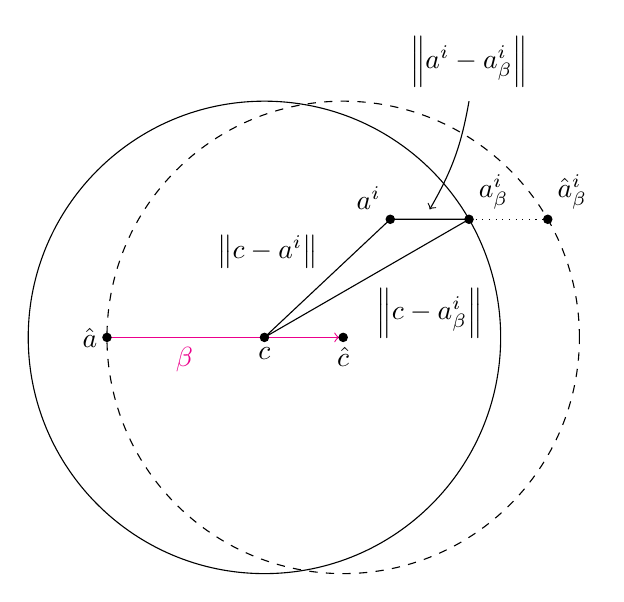
\begin{tikzpicture}
        % lines
        \draw (0,0) -- (1.598, 1.5) node[midway, above left]{$\norm{c-a^i}$} -- (2.598, 1.5) -- cycle node[midway, below right]{$\norm{c-a^i_\beta}$};
        \draw[dotted] (2.598, 1.5) -- (3.598, 1.5);
        
        \draw[->, color=magenta] (-2,0) -- (0.95,0) node[pos=0.3333, below]{$\beta$};
        
        % points
        \draw[fill] (0,0) circle (1.5pt) node[below] {$c$};
        \draw[fill] (-2,0) circle (1.5pt) node[left]{$\hat{a}$};
        \draw[fill] (1,0) circle (1.5pt) node[below]{$\hat{c}$};
        
        \draw[fill] (1.598, 1.5) circle (1.5pt) node[above left]{$a^i$};
        \draw[fill] (2.598, 1.5) circle (1.5pt) node[above right]{$a^i_\beta$};
        \draw[fill] (3.598, 1.5) circle (1.5pt) node[above right]{$\hat{a}^i_\beta$};
        
        % balls
        \draw (0,0) circle (3);
        \draw[dashed] (1,0) circle (3);
        
        % labels
        \node at (2.598, 3.5) {$\norm{a^i-a^i_\beta}$};
        \draw[->] (2.598, 3) to[bend left=10] (2.098, 1.625);
        
    \end{tikzpicture}
    \caption{Visual Aid for Proposition \ref{imp heuristic feasibility}}
    \label{vis aid feasibility}
\end{figure}
\subsubsection{Complexity}

The complexity of the DCSSH is easy to determine. Referring to Algorithm \ref{fig:dcssh}, on line 1 we have a loop over each data point which runs in $O(n)$ time. On lines 4 through 6 we have a \texttt{for} loop which runs $n$ many times, with the operations on lines 5 and 6 both being $O(d)$ as they are each single operations on $d$-dimensional vectors, so overall this loop runs in $O(nd)$ time. On lines 7 and 8 we find the minimum and maximum of two lists respectively, again $O(n)$. Finally, on line 8, a single operation on $d$-dimensional vectors runs in $O(d)$ time. Our dominating term is then $O(nd)$.
\subsection{Direction-Constrained MEB Heuristic}
For a visual aid to this derivation please refer to Figure \ref{fig:dcmeb}. Consider $B(\hat{c},\hat{r})$. Similarly to the DCSSH, for an improving direction we choose the furthest point in $\A$ from $\hat{c}$, $\hat{a}=\arg\max_{a\in\A}\norm{\hat{c}-a}$, and let $\beta=\hat{a}-\hat{c}$ be this direction. Note that this is the negative of $\beta$ used in the derivation of the DCSSH, as we are now considering the direction $\hat{c}\to\hat{a}$. Now, instead of calculating distances between each point in data and the surface of the ball to find a feasible step length from $\hat{c}$ towards $\hat{a}$, we formulate an optimization model to find an optimal step length such that the new ball still contains all data, but has a smaller radius.

We modify the optimization model for the MEB problem, adding the constraint that $c$ must lie on the direction $\beta$ from $\hat{c}$. It is possible to formulate this exactly using the constraint $c=x(\hat{c}+\beta)$, however a better formulation is to consider a variable $x\in\mathbb{R}^{\geq0}$, then write $c=\hat{c}+\beta x$. Obviously $\hat{c}$ is a constant vector so this reduces the problem of finding the new $c$ to that of finding the optimal solution to one variable $x$, as opposed to $d$ many decision variables for each element of the vector $c$. The optimization model for the DBMEB problem is as follows:
\begin{center}
    \begin{tabular}{CCC}
        \displaystyle\min_{x,r} & r \\
        \text{s.t.} & \norm{\hat{c}+\beta x - a^i} \leq r & i=1,\ldots,n \\
        & x\geq0
    \end{tabular}
\end{center}

By setting $\gamma=r^2$, $\alpha^i=\hat{c}-a^i$ for $i=1,\ldots,n$, and squaring the norm constraints, we get the following quadratic model:
\begin{center}
    \begin{tabular}{CCC}
        \displaystyle\min_{x,\gamma} & \gamma \\
        \text{s.t.} & \beta^T\beta x^2 + 2\alpha_i^T\beta x + \alpha_i^T\alpha_i \leq \gamma & i=1,\ldots,n \\
        & x\geq0
    \end{tabular}
\end{center}

This model has $n+1$ constraints and most crucially, 2 decision variables. This makes the model extremely computationally easy to solve by modern solvers such as Gurobi. The DCMEB heuristic is then to simply solve the DCMEB, given a data set $\A$ and initial ball $B(\hat{c},\hat{r}$, using the solutions of the solved DCMEB problem for the new ball.

\begin{algorithm}
    \KwIn{Data set $\A$, Ball $B(\hat{c},\hat{r}$)}
    \KwOut{Ball $B(c,r)$}
    $\hat{a}:=\arg\max_{a\in\A}\norm{\hat{c}-a}$\;
    Let $x$, $r$ be the solutions returned by solver for the DCMEB problem for $B(\hat{c},\hat{r})$\;
    $c:=c+x(\hat{a}-\hat{c})$\;
    \KwRet{$B(c,r)$}\;
    \caption{Direction-Constrained MEB Heuristic}
\end{algorithm}

\begin{figure}
    \centering
    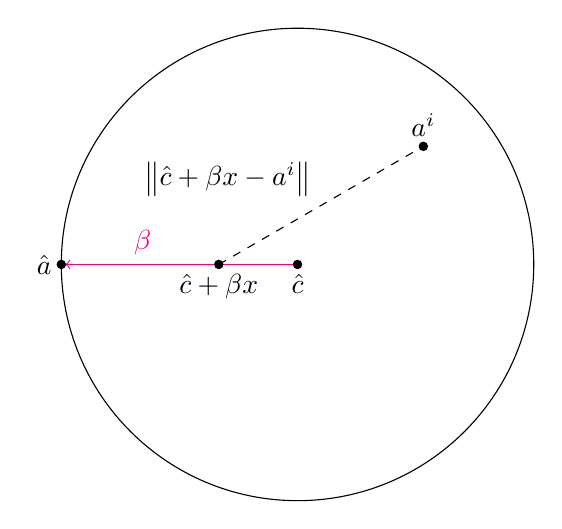
\begin{tikzpicture}
        % lines
        \draw[->, color=magenta] (0,0) -- (-2.95,0) node[pos=0.6666, above]{$\beta$};
        \draw[dashed] (-1,0) -- (1.598, 1.5) node[midway, above left]{$\norm{\hat{c}+\beta x - a^i}$};
        % points
        \draw[fill] (0,0) circle (1.5pt) node[below]{$\hat{c}$};
        \draw[fill] (-3,0) circle (1.5pt) node[left]{$\hat{a}$};
        \draw[fill] (1.598, 1.5) circle (1.5pt) node[above]{$a^i$};
        \draw[fill] (-1,0) circle(1.5pt) node[below]{$\hat{c}+\beta x$};
        
        % ball
        \draw (0,0) circle (3);
    \end{tikzpicture}
    \caption{Visual Aid for Direction-Constrained MEB}
    \label{fig:dcmeb}
\end{figure}
% =============================================================================
% Chapter 4
% =============================================================================
\chapter{Implementation and Experiments}\label{implementation}
\section{Code Implementation}
\subsection{Data}

\section{Experiments}
\subsection{Methodology}
\subsection{Exact Model}\label{exact benchmarks}
\subsection{Construction Methods}
\subsubsection{Relaxation-based Heuristic}
\subsubsection{Shrinking Heuristic}
\subsubsection{Shenmaier's Approximation}

\subsection{Improvement Heuristics}
\subsubsection{Direction-Constrained Single Step Heuristic}
\subsubsection{Direction-Constrained MEB}

\section{Discussion}

% =============================================================================
% Chapter 5
% =============================================================================
\chapter{Conclusion}

% =============================================================================
%the entries have to be in the file literature.bib
\bibliography{literature}
\clearpage

\appendix
\section*{Appendices}
\addcontentsline{toc}{section}{Appendices}

\section{An Appendix}
\label{app:one}

Some stuff.
\clearpage

\section{Another Appendix}
\label{app:two}

Some other stuff.

\end{document}
